\chapter{Results}
\label{chap:results}

The results of the simulation runs were averaged together and are shown in Table~\ref{tab:avgResults} and plotted in Figure~\ref{fig:averages}.  Standard deviations are included in table as $\pm$ values next to their corresponding averages.  The complete raw time data per world and per communication range can be found in Appendix~\ref{sec:raw_data}.


\begin{table}[H]
	\caption{Average time to complete objectives}
	\centering
%	\rowcolors{1}{lightgray}{white}
	\label{tab:avgResults}
%	\begin{tabular}{|p{1.1cm}|p{1.75cm}|p{1.75cm}|p{1.5cm}|}
	\begin{tabular}{c c c c}
		\hline
		\parbox[c]{1.1cm}{\centering Comm.\\Range\\ \%} & \parbox[c]{1.75cm}{\centering Average\\time all\\detected\\(s)} & \parbox[c]{1.75cm}{\centering Average\\time all\\destroyed (s)} & \parbox[c]{1.5cm}{\centering Average\\time\\world\\known\\(s)}\\
		\hline
		100 & 116 $\pm$ 52 & 206 $\pm$ 58  & 61 $\pm$ 29  \\
		20  & 151 $\pm$ 62 & 239 $\pm$ 53  & 90 $\pm$ 68  \\
		10  & 116 $\pm$ 53 & 231 $\pm$ 77  & 95 $\pm$ 48  \\
		5   & 161 $\pm$ 93 & 294 $\pm$ 85  & 129$\pm$50 \\
		2   & 221 $\pm$ 90 & 434$\pm$105 & 238$\pm$112 \\ \hline
	\end{tabular}
\end{table}

Table~\ref{tab:avgResultsRatio} shows the ratios of performance between the test cases.  The $10\%$ and $20\%$ range cases at worst take $155\%$ of the time required by perfect global network baseline.

\begin{table}[H]
	\caption{Ratio of time to complete objectives compared to 100\% range}
	\centering
	%	\rowcolors{1}{lightgray}{white}
	\label{tab:avgResultsRatio}
	%	\begin{tabular}{|p{1.25cm}|p{1.5cm}|p{1.75cm}|p{1.5cm}|}
	\begin{tabular}{c c c c}
		\hline
		\parbox[c]{1.25cm}{\centering Comm.\\Range\\ \%} & \parbox[c]{1.5cm}{\centering Average\\time all\\detected\\ratio} & \parbox[c]{1.75cm}{\centering Average\\time all\\destroyed\\ratio} & \parbox[c]{1.5cm}{\centering Average\\time\\world\\known\\ratio}\\
		\hline
		100 & 1.0   & 1.0   & 1.0   \\
		20  & 1.299 & 1.163 & 1.481 \\
		10  & 1.0   & 1.122 & 1.547 \\
		5   & 1.393 & 1.43  & 2.112 \\
		2   & 1.902 & 2.11  & 3.895 \\ \hline
	\end{tabular}
\end{table} 


A more interesting view of the data is shown via Tukey style boxplots in Figures~\ref{fig:detectBoxPlot}, \ref{fig:destroyedBoxPlot}, and \ref{fig:knownBoxPlot} comparing the time to detect all targets, the time to destroy all targets, and the time to confidently know the whole world respectively.  The first and third quartiles of the metric data recorded across all 10 words is bounded by the blue boxes in the figures.  The red lines are the median values and the red dots are the average.  The whiskers are set to the nearest datum still within 1.5 times the interquartile range (also called the midspread or middle 50\%).  The blue dots are outliers beyond the interquartile range.

\end{multicols*}

\begin{figure}[H]
	\centering
	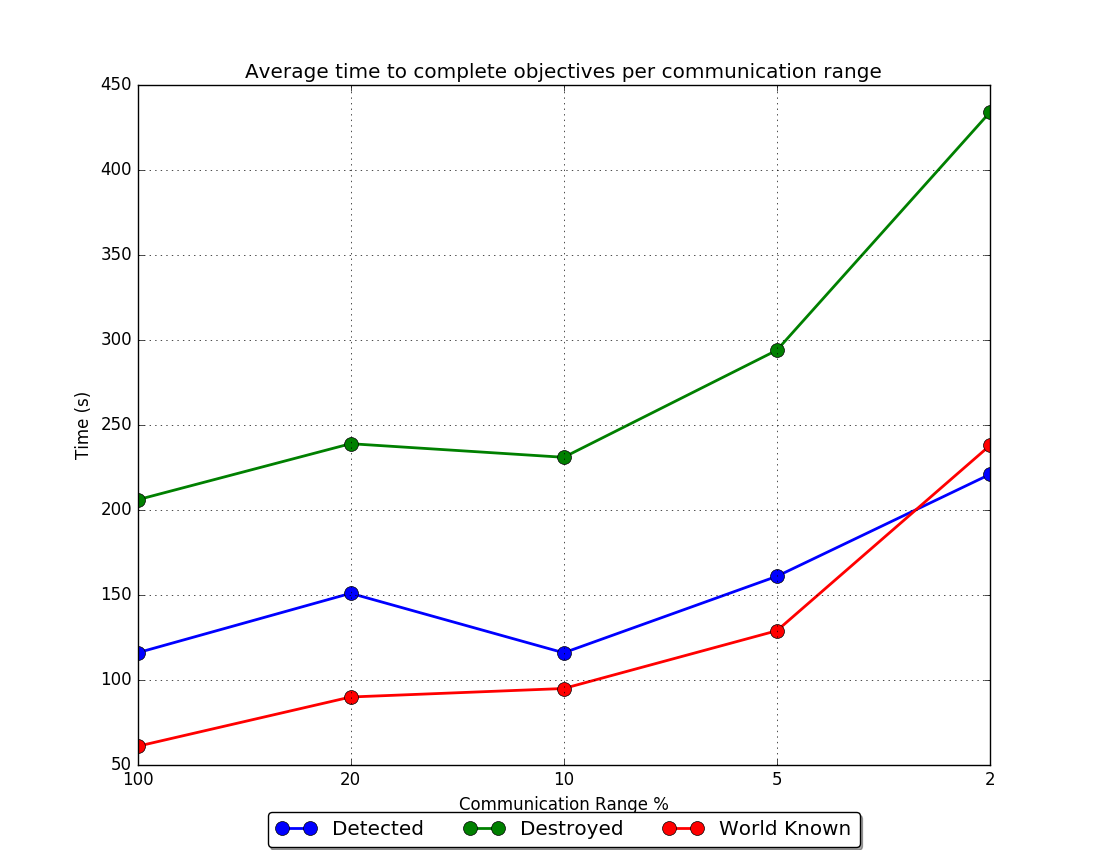
\includegraphics[width=\linewidth,height=3.5in,keepaspectratio=false]{averages.png}
	\caption{Average time to complete objectives per communication range}
	\label{fig:averages}
\end{figure}

\begin{figure}[H]
	\centering
	\includegraphics[width=\linewidth,height=3.5in,keepaspectratio=false]{detected_box.png}
	\caption{Boxplot for time to detect all targets per communication range}
	\label{fig:detectBoxPlot}
\end{figure}

\begin{figure}[H]
	\centering
	\includegraphics[width=\linewidth,height=3.5in,keepaspectratio=false]{destroyed_box.png}
	\caption{Boxplot for time to destroy all targets per communication range}
	\label{fig:destroyedBoxPlot}
\end{figure}

\begin{figure}[H]
	\centering
	\includegraphics[width=\linewidth,height=3.5in,keepaspectratio=false]{known_box.png}
	\caption{Boxplot for time to know whole world per communication range}
	\label{fig:knownBoxPlot}
\end{figure}

\begin{multicols*}{2}


%-------------------------------------------------------------------------

\chapter{Discussion}
\label{chap:discussion}

The $100\%$ communication range case serves as a comparative baseline against a perfect global communication network.  In this case all UAVs are able to communicate with all other UAVs at all times.  As expected a perfect global and centralized communication network performs better than networks with limited ranges.  The interesting point of comparison is that the $10\%$ and $20\%$ range cases come very close or match the $100\%$ case in all performance metrics. 

The similar performances can be attributed to the density of UAVs in the swarm.  This simulation used 5 UAVs in a 2.5 by 2.5$Km$ world.  Assuming the UAVs are equally spaced across the world to maximize communication coverage then Table~\ref{tab:worldCommsRngCoverage} shows how much of the world is covered in each test case.  The \textit{Physical Comm. Range} is the maximum distance across the world ($3.54Km$) times the \textit{Communication Range \%} yielding the maximum communication distance between UAVs for the test case.  The \textit{Maximum Possible Coverage} is the sum of the circular coverage areas of the 5 UAVs.  The \textit{Percent of World Area} is the the \textit{Maximum Possible Coverage} divided by the total area of the mission world converted to a percentage.  Since the UAVs are equally spaced for best possible communications coverage in these calculations the \textit{Percent of World Area} is a theoretical upper limit and will never be achieved in any practical means.

\begin{table}[H]
	\caption{World communication coverage percentage}
	\centering
	%	\rowcolors{1}{lightgray}{white}
	\label{tab:worldCommsRngCoverage}
	%	\begin{tabular}{|p{1.25cm}|p{1.5cm}|p{1.75cm}|p{1.5cm}|}
	\begin{tabular}{c c c c}
		\hline
		\parbox[c]{1.25cm}{\centering Comm.\\Range\\ \%} & \parbox[c]{1.5cm}{\centering Physical\\Comm.\\Range\\($Km$)} &  \parbox[c]{1.75cm}{\centering Maximum\\Possible\\Coverage\\($Km^{2}$)} & \parbox[c]{1.5cm}{\centering Percent\\of\\World\\Area\\(\%)}\\
		\hline
		100 & 3.54 & 196.35 & 3141.59 \\
		20  & 0.71 & 7.85   & 125.66  \\
		10  & 0.35 & 1.96   & 31.42   \\
		5   & 0.18 & 0.49   & 7.85    \\
		2   & 0.07 & 0.08   & 1.26    \\ \hline
	\end{tabular}
\end{table} 

Assuming theoretical best positioning the $20\%$ and $10\%$ cases can cover 125\% and 31\% of the world simultaneously respectively. Since the UAVs are constantly moving these coverage values are never reached.  However, their actual coverage values are sufficiently high that they randomly come in contact with each other frequently to enable the sharing of information.  This lets the $20\%$ and $10\%$ cases achieve similar performance metrics to the $100\%$ range baseline.  Conversely, even the theoretical best communication coverage of the world for the $5\%$ and $2\%$ is a very low percentage and makes it difficult for those test cases to share belief data and coordinate.

The boxplots in figures~\ref{fig:detectBoxPlot} - \ref{fig:knownBoxPlot} display a gradual degradation in the performance metrics as communication ranges decrease.  In general all of test cases are roughly equal in performance to each other except the $2\%$ case.  The $10\%$ case in figure~\ref{fig:detectBoxPlot} looks odd in the plot due to the upper data points just barely crossing the threshold of the 1.5 interquartile range limit for a Tukey style boxplot.  This makes the upper two data points look like outliers in that dataset, however they fall in line  with the other datasets so they are not really abnormal. 

Given the high theoretical upper limit for \textit{Percent of World Area} covered by the $20\%$ and $10\%$ test cases in Table~\ref{tab:worldCommsRngCoverage} it can be expected that those cases perform well since there is a high probability that at least one other swarm member is in communication range.  The $5\%$ test case produced a surprising performance.  At best the 5 UAVs can only cover $7.85\%$ of the world at once yet it performed as well as the larger communication cases in its \textit{Time to detect all targets} and \textit{All world known} metrics.  This means despite the communication handicap the swarm was able to efficiently scan and survey the mission world.  The $5\%$ case suffered in the \textit{Time to destroy all targets} metric but still performed relatively well.  The performance drop can be directly attributed to the communication restriction.  In this model in order for a target to be attacked two swarm members must be in communication's range of each other and at least one of them must be an attack platform.  The simulation logs show that many times the Monitoring platforms timed out and let their targets go since an available Attack platform was not in communications range or able to be within range by the time a 3rd UAV carried the attack request to the rest of the swarm.

The $2\%$ communication's range test case is near useless for mission planning purposes but provides a set of worst case data points.  The communications range is so insignificantly small compared to the size of the world area and the number of UAVs that the outcome is essentially random if swarming behaviors occur or not.  Table~\ref{tab:avgResults} shows an average detection time of 221 seconds and a standard deviation of 90s which is 40\% of the average value.  A $\pm$ $40\%$ swing around the average is far to unreliable for mission planning purposes.

It is interesting to note that the better performing ends (lower times) of the $2\%$ case still manage to complete the mission objectives and overlap with the performance of the larger test cases for all metrics. Using the simulation's graphical interface it was verified that the worst performing simulations had very few interactions amongst the swarm members while the better performing simulations had more interactions.  Hence, the $2\%$ test case is useful for two purposes.  One is that it shows that the algorithm can complete a mission even when members of the swarm essentially act as solo agents but it takes much more time.  The second purpose is that it indirectly highlights the benefits of swarming versus solo agents.  When swarming interactions did occur the mission objectives were completed much more quickly than when swarming interactions did not occur.

%The $20\%$ and $10\%$ cases are not as heavily pressured as the shorter range cases to react to targets immediately.  These longer range cases can afford to wait for the most appropriate UAV to become available for the monitor and strike tasks so their average time to Destroy is roughly double that of their time to Detect everything.  The UAVs do not have to focus as much time on search and exploration tasking to maintain world certainty and keep Shannon entropy to a minimum.



%In contrast, the shorter range cases must react quickly once a target is found otherwise there is a strong possibility it will be lost.  This explains why the average time for Detections and World Known are near equal in the $5\%$ case with the average Destroyed time not far behind.  Once a target is seen it is immediately destroyed.

%The $2\%$ case shows a similar trend in the time necessary for Detecting and World Known but the Destroyed time is drastically slower.  This is likely because the much shorter range requires the UAVs to frequently give up Monitoring a target since no strike platform is around before the Monitor time out occurs.  In the $2\%$ case the only time a target is struck is when 2 UAVs happen to be near each other when the target is found or a strike UAV happens to be exploring a part of the world it thinks is highly uncertain.  The strike platform will synchronize with the Monitoring UAV and immediately begin the attack process, assuming it has munitions available, otherwise it will have to relay the message to someone else in the swarm.

Within the performance limits and size of the swarm in these simulations we can see that there is no absolute need for every member of a swarm to be able to reach all others in a global fashion.  In practice with standard radio communication  equipment this is actually undesirable because the UAVs will constantly be jamming each other inadvertently.  The standard trade off is finding a suitable transmission range that allows sufficient bandwidth and world coverage between members of the swarm.  Another real world constraint on radio transmissions is the desire to remain undetected.  By limiting our transmission range and power we can limit the range of detectability by enemy radio detection sensors.

Within the constraints of this simulation we can drop the transmission range down to $10\%$ of the maximum world range with almost no detrimental affects on overall mission performance.  If some performance degradation is acceptable we can further reduce the communication range requirements to $5\%$.  It seems extreme but is also possible to still complete the mission with only a $2\%$ communication range albeit with a much longer mission duration and a high risk of failure.

\section{Limitations of the Study}
There are a few results where the swarm was unable to complete the mission.  World 3 was a problem for the $100\%$, $10\%$, and $2\%$ cases.  World 3 can be seen in Figure~\ref{fig:world3}.  There is a static target located at row 9 column 0.  The best approach angle for striking the static target is $\pm$ $45^{\circ}$.  In this physically literal edge case those approach angles puts the UAVs on a trajectory outside of the world.  Therefore the UAVs will attempt strikes at very poor angles from the target's backside instead.  The simulation logs show that many shots are taken at this target and miss.  Eventually all of the strike platforms run out of munitions on this target unless they get very lucky.  This result is a limitation of the simulation's random generation nature.  A real world mission analyst would expand the mission area to allow for a better strike angle against this target.  The simulation does not account for accumulating damage.  Every strike is a boolean draw to decide if a target is destroyed or not.  So even though in the simulation dozens of shots were fired at the target it is still considered alive and well.  In the real world dozens of shots would have likely caused significant if not fatal damage to the target even when fired from an undesirable angle.

Communication range case of $5\%$ failed to complete world 4 and case $2\%$ failed to complete world 9.  In both cases a mobile target survived.  The logs show that the Attack platforms and the Monitoring platforms were not in communication range in both cases.  This compounded into multiple problems and possible failure issues.  The strike UAVs, who are the only armed aircraft, have very poor sensors compared to the ISR platforms.  The Attack platforms have a hard time finding and tracking mobile targets with these poor sensors.  Since the Attack and Monitor aircraft were not in communication range the Attack platforms usually had out-dated information about the target's location.  Therefore the attack platform flew to the target's previous location and the attack aircraft's poor sensors could not detect the target in the surrounding areas.  Eventually the attack platform would give up since it could not find the target.

Another compounding issue in these short communication range cases is when the Monitoring UAVs were strike platforms instead of ISR platforms.  In these cases a strike platform would happen upon a target but no ISR platforms were able to hear about the target announcement.  Therefore the strike platform would perform the Monitoring task and do a poor job of it.  It would follow the mobile target while requesting for a second strike platform to perform the Attack task.  When a strike platform began performing the Attack it would suffer from the same poor sensor issues as the Monitoring platform, leading to many shots at where a target ``was'' instead of where it really ``is.''


\section{Directions for Future Work}
As shown by simulation the Implicit Territorial Swarming algorithm is functional but there is always room for improvement.  In this scenario all aircraft had an equal communication range.  An interesting excursion would be to model varying communication ranges amongst individuals in the swarm.  Similarly, the addition of communication relay payloads whose sole purpose is to relay data from one part of the swarm to another would add an interesting dynamic.

There is room for enhancement in the rules for swarm cooperation.  Currently the same platform cannot Monitor and Attack at the same time even when both tasks encompass the same target.  This would certainly effect the effectiveness of the extremely small communication range cases.  Another interesting concept is the idea of an ``interested bidder'' for tasks.  In this case a platform is currently engaged in performing task A but hears about new task B.  The UAV is very well suited for task B but it should not abandon its current task A until someone can take it over.  As is some other UAV will pick up task B, but it may do the job poorly compared to the UAV stuck on task A.  With this new concept the busy UAV could announce that it is very interested in task B and that anyone who can closely match its score on task A can takeover the work for task A.  Other UAVs hearing about the interested bidder might change their behaviors to help relieve the UAV on task A or temporarily delay their execution of task B to see if the UAV on task A gets relieved.

The weighted average used for merging belief data in section~\ref{sec:uavBelief} is brought about by a limitation of the representation of world uncertainty.  Future work could find new ways of measuring uncertainty or weighing in the expertise of a sensor in the belief model so that a more automated merging algorithm can be used.  As is, the operator must provide a configuration value to weight the merging of data which adds to the burden of using this model.

The application of the model and analysis of the results provides a rough procedural outline for exploring the trade space between many factors in swarm design.  Future work could vary the number of targets, the number of UAVs, the ratio of strike to ISR platforms, and the types of payloads.